\section{Introduction}
Ce document contient les spécifications détaillées des exigences du projet ainsi que l'analyse faite pour chaque tâches. Ces deux étapes sont essentielles pour partir dans la bonne direction dès le début de chaque itération. 
\section{Analyse}
	\subsection{ Aperçu global}
	 \EPSFIGTEXTWIDTH{../comon/figures/apercu.pdf}{Vue globale des fonctionnalités du produit}{apercuGlob}
	\subsection{Use case}
	 \EPSFIGTEXTWIDTH{../comon/figures/UC.pdf}{Diagramme des cas d'utilisation de l'application}{UC}
	 Les fiches descriptive du chapitre~\ref{exigenceFoction} détail les cas d'utilisation.
	\subsection{Description des utilisateurs}
		\textbf{Professeurs :} représente les professeurs de l'USJ.\\[0.2cm]
		\textbf{Étudiants :} représente les étudiants de l'USJ.\\[0.2cm]
		\textbf{Visiteurs :} représente les visiteurs et les personnes non enregistré de l'USJ.\\[0.2cm]
		\textbf{WebServices :} représente les web services de l'\gls{USJ} qui nous permettent d'accéder aux informations de la base de données.\\[0.2cm]
		\textbf{FS\_Local :} représente les données stocké en local sur l'appareil.\\[0.2cm]
	\subsection{Faisabilité}
		\textbf{UC\_0  Naviguer}  L'\gls{iOS} d'afficher différentes vues et naviguer d'une façon simple entre elles. Ce cas d'utilisation et \textbf{100 \%  faisable}.\\[0.2cm]
		\textbf{UC\_1  Paramétrage}  L'\gls{iOS} permet de stocker des paramètres d'application d'une façon simple. Ce cas d'utilisation est \textbf{100 \%  faisable}.\\[0.2cm]
		\textbf{UC\_2  Login}  L'\gls{iOS} permet d'accéder au web services à travers différentes classes et ces classes prennent en charge la gestion des sessions pour le login.Ce cas d'utilisation est \textbf{100 \%  faisable}.\\[0.2cm]
		\textbf{UC\_3  Carte}  La librairie MapKit livrer avec l'\gls{iOS} permet d'afficher des cartes en se basant sur la base de données de google map.Il est aussi possible d'ajouter des annotations à des emplacement précis de la carte. Cette librairie est utilisable gratuitement et librement, elle répond à tout les besoins de notre application.Il es aussi possible grâce au gps des appareils de détecter la position de l'utilisateur.  Ce cas d'utilisation est \textbf{100 \%  faisable}.\\[0.2cm]
		\textbf{UC\_4  AfficherNews}  Les outils à disposition permettent d'effectuer aisément ce genre de tâches  .Pour le détail des news, il est possible d'intégrer un navigateur web dans l'application. Ce cas d'utilisation est \textbf{100 \%  faisable}.\\[0.2cm]
		\textbf{UC\_5 AfficherAnnuaire}  L'annuaire est disponible via les web services, le but ici est de le présenter d'une façon pratique à l'utilisateur. Ce cas d'utilisation est \textbf{100 \%  faisable}.\\[0.2cm]
		\textbf{UC\_6 AfficherHorraire}  L'annuaire est disponible via les web services, le but ici est de le présenter d'une façon pratique à l'utilisateur. Ce cas d'utilisation est \textbf{100 \%  faisable}.\\[0.2cm]
\section{Spécification des exigences }
	\subsection{Spécification des interfaces}
		\textbf{Interfaces utilisateur}  
			Aucune ligne graphique est imposé, la seul contrainte est d'utiliser les logos originaux de l'école.\\[0.2cm]
		\textbf{Interfaces Hardware} 
			L'iPhone et l'iPad possède un écran tactile qui sera utilisé pour interagir avec l'utilisateur. D'autre capteurs comme le gyroscope,caméra ou accéléromètre sont disponible sur l'appareil mais ne seront pas utilisé pour ce projet. \\
			L'iPhone et l'iPad se connectent à internet via le 3Gs et le WIFI pour récupérer les données des web services.\\[0.2cm]
	 	\textbf{Interfaces Software} 
			L'application utilise les web services de l'\gls{USJ} pour accéder au base de données. Les web services n'existant pas avant la création de l'application, il faut définir la manière de communiquer avec les web services. Pour ce faire, M.Medawar fournit un fichier XML ainsi que le XML Schema correspondant du résultat que l'on attend d'un web service et le service informatique de l'USJ fournira ce service.  L'annexe E(/Documentation/Annexes/E) contient tout les fichiers XML et XML Schema fournis au service informatique. \\
			\todo{describe web service url and methode}
			  \begin{lstlisting}[language=XML,caption = Exemple de code XML fournit au service informatique de l'USJ]
<?xml version="1.0" encoding="UTF-8"?>
<!-- Resultat de l'appel https://www.url.com/webSerivice.php 
    avec les parametres en POST suivant:
    usr = 'elias.medawar'
    pwd = '1234'
    op  = 'testCommunication'
-->
<response xmlns:xsi="http://www.w3.org/2001/XMLSchema-instance"
 xsi:noNamespaceSchemaLocation="schemaTest.xsd">
    <!-- Une reponse valide pour tester la communication -->
    <status>0</status>
    <usrGroup>2</usrGroup>
    <commentaire><![CDATA[Communication possible]]></commentaire>
</response>
			\end{lstlisting}

 \begin{lstlisting}[language=XSD,caption = Exemple de XML Schema fournit au service informatique de l'USJ]
<?xml version="1.0" encoding="UTF-8"?>
<xs:schema xmlns:xs="http://www.w3.org/2001/XMLSchema" elementFormDefault="qualified">
  <xs:element name="response">
    <xs:complexType>
      <xs:sequence>
        <xs:element ref="status"/>
        <xs:element ref="usrGroup"/>
        <xs:element ref="commentaire" minOccurs="0" maxOccurs="10"/>
      </xs:sequence>
    </xs:complexType>
  </xs:element>
  <xs:element name="status">
    <xs:simpleType>
      <xs:restriction base="xs:int">
        <xs:enumeration value="-2"></xs:enumeration><!-- Intenrnal error in the webservices.KO -->
        <xs:enumeration value="-1"></xs:enumeration><!-- Wrong password or login.KO -->
        <xs:enumeration value="0"></xs:enumeration><!-- Successful execution.OK -->
      </xs:restriction>
    </xs:simpleType>
  </xs:element>
  <xs:element name="usrGroup">
    <xs:simpleType>
      <xs:restriction base="xs:int">
        <xs:enumeration value="0"></xs:enumeration><!-- User login is not a registred, asume that it's a visitor -->
        <xs:enumeration value="1"></xs:enumeration><!-- User login correspond to a professor -->
        <xs:enumeration value="2"></xs:enumeration><!-- User login correspond to a student -->
      </xs:restriction>
    </xs:simpleType>
  </xs:element>
  <xs:element name="commentaire" type="xs:string"/>
</xs:schema>
			\end{lstlisting}

	\textbf{Protocoles de communications:} L'application communique via HTTPS avec les web services . \\[0.2cm]
	\subsection{Exigences fonctionnelles \label{exigenceFoction}}
	
		\subsubsection{Naviguer}
				L'utilisateur doit pouvoir naviguer dans les différents menu de l'application.\\[0.2cm]
				\begin{longtable}{|l|p{10cm}|}
					\hline \textbf{Nom du Use Case} & Naviguer \\ 
					\hline \textbf{Ref} & UC\_0  \\ 
					\hline \textbf{Déclencheur} & L'utilisateur démarre l'application \\
					\hline \textbf{Précondition} &  \\
					\hline \textbf{Scénario nominal} & 
					\begin{enumerate}
						\item Le système affiche le menu de l'application
						\item L'utilisateur clique sur  un élément du menu.
						\item Le système affiche la vue correspondante au bouton cliquer .
						\item L'utilisateur effectue la tâche dont il a besoin à l'aide de la vue afficher.
						\item L'utilisateur revient sur la page du menu de l'application.
						\item Recommencement au point 2 du UC.
					\end{enumerate}
					\\ 
					\hline \textbf{Enchaînements alternatifs} &  
						Commence au point 4 du scénario  nominale(sur IPad)
						\begin{enumerate}
							\item L'utilisateur  clique sur un autre élément du menu.
							\item Continue au point 3 du scénario nominale.
						\end{enumerate}
						
					\\
					\hline \textbf{Status actuel} & Planifié:\CheckedBox , Implémenté:\CheckedBox , Testé: \CheckedBox , Validé: \CheckedBox \\
					\hline 
				\end{longtable} 
		\subsubsection*{Besoin graphique}
				\begin{figure} 
					\centering 
					\subfigure[Navigation sur IPhone]{\label{fig:gull}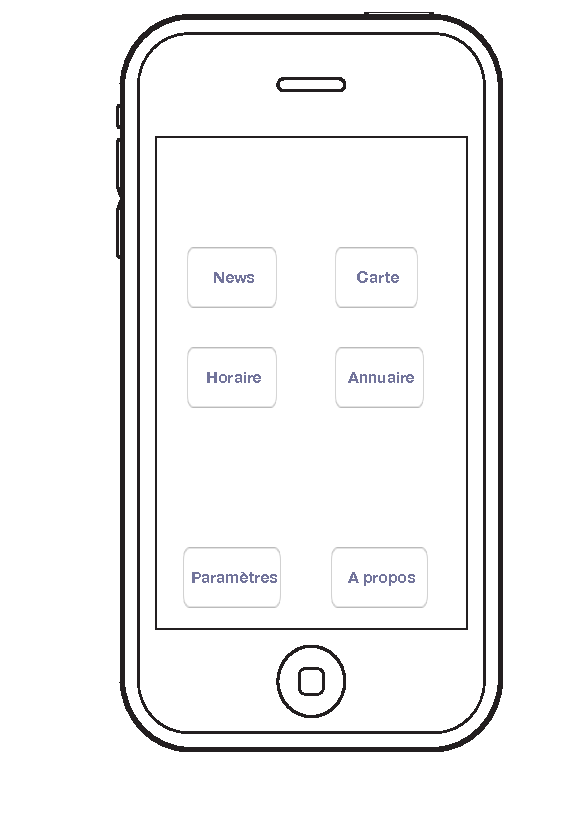
\includegraphics[width=0.3\textwidth]{../comon/figures/MainMenuIPhone.pdf}} 
					\subfigure[Navigation sur IPad]{\label{fig:tiger}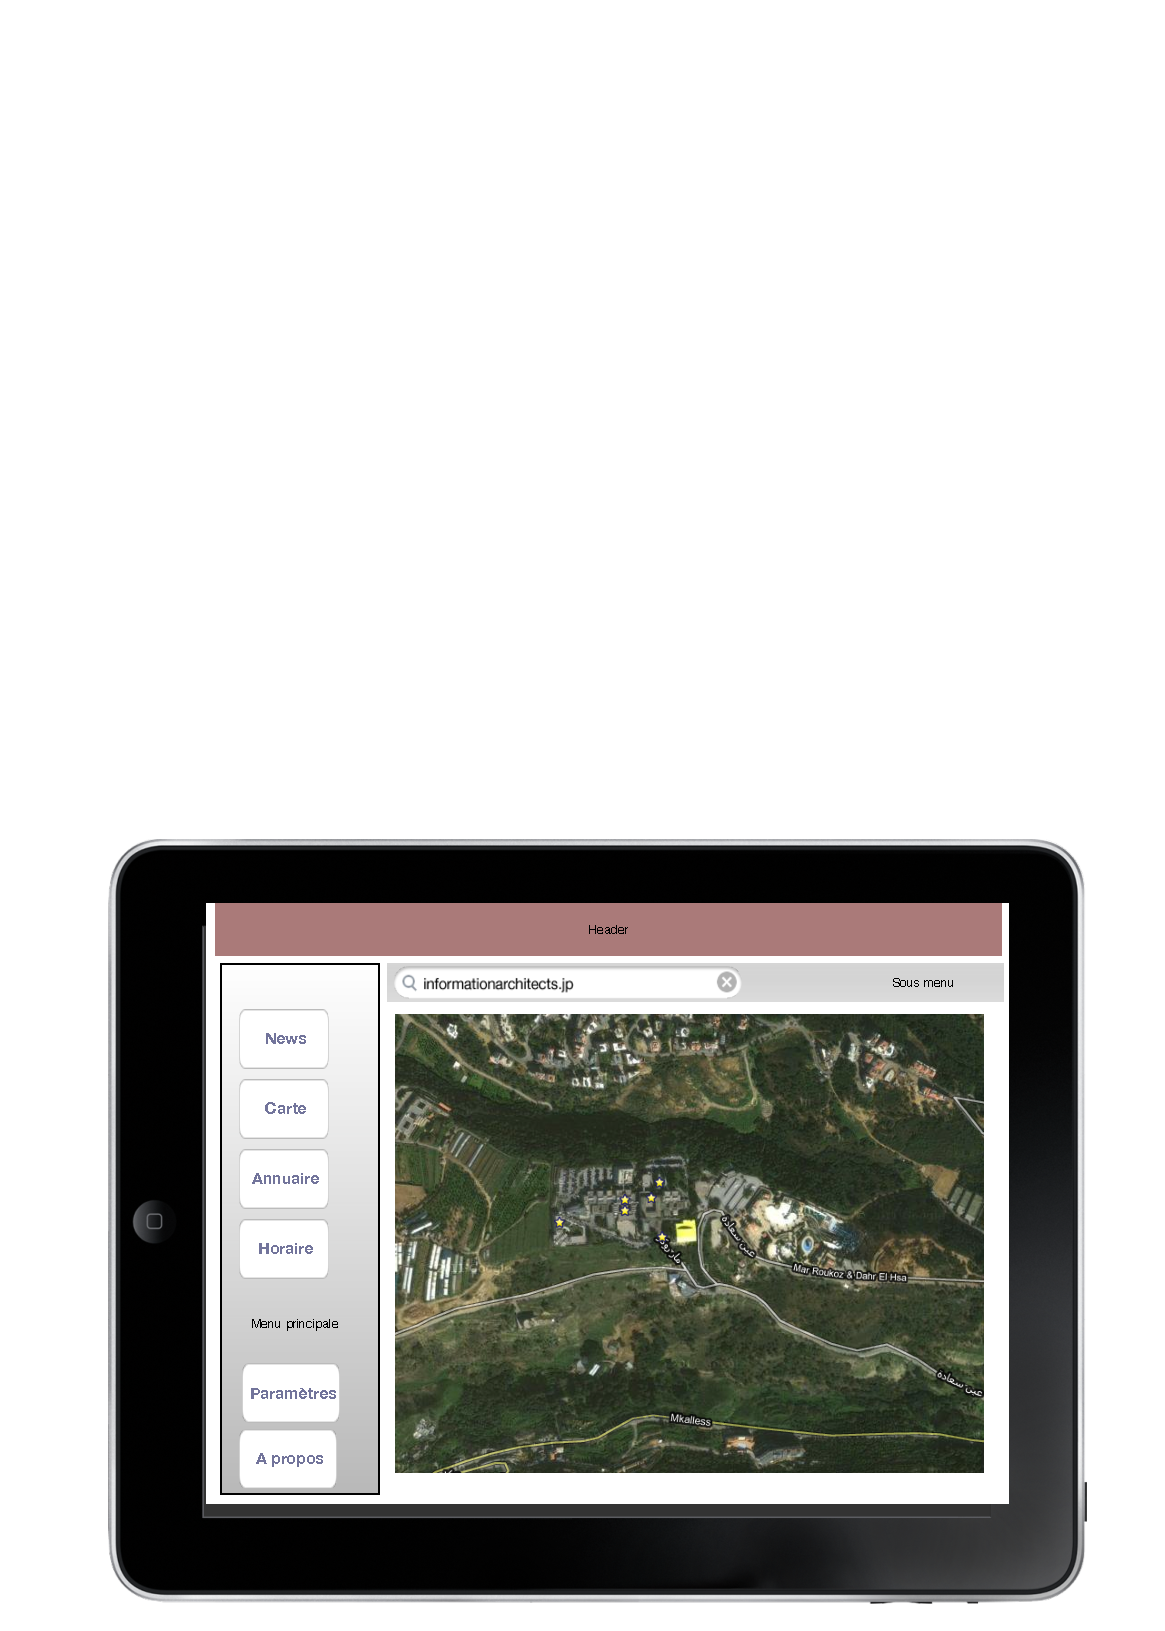
\includegraphics[width=0.6\textwidth]{../comon/figures/MainMenuIPad.pdf}} 
				\end{figure}
				
				
				
		\subsubsection{Paramétrer l'application}
			L'utilisateur doit pouvoir choisir les paramètres de l'application et les sauvegarder.\\[0.2cm]
			\begin{longtable}{|l|p{10cm}|}
				\hline \textbf{Nom du Use Case} & Paramétrage \\ 
				\hline \textbf{Ref} & UC\_1  \\ 
				\hline \textbf{Déclencheur} & L'utilisateur clique sur le bouton paramètre \\
				\hline \textbf{Précondition} &  \\
				\hline \textbf{Scénario nominal} & 
				\begin{enumerate}
					\item Le système restaure les valeurs des paramètres depuis le fichier de configuration et les affiche.
					\item L'utilisateur choisit une option qu'il désire modifier.
					\item L'utilisateur modifie la valeur.
					\item \label{uc1Mod}L'utilisateur confirme qu'il a finit de modifie la valeur
					\item Le système sauvegarde la valeur.
				\end{enumerate}
				\\ 
				\hline \textbf{Enchaînements alternatifs} &  \\
				\hline \textbf{Status actuel} & Planifié:\CheckedBox , Implémenté:\CheckedBox , Testé: \CheckedBox , Validé: \CheckedBox \\
				\hline 
			\end{longtable} 
		\subsubsection*{Besoin graphique}
		\EPSFIGTEXTWIDTH{../comon/figures/WierframeIPhoneSettings.pdf}{Wireframe illustrant les modifications des paramètres sur l'iPhone}{wireIPhoneSett}
		\EPSFIGTEXTWIDTH{../comon/figures/WierframeIPadSettings.pdf}{Wireframe illustrant les modifications des paramètres sur l'iPad}{wireIPhoneSett}

		\subsubsection{Login}
			Pour accéder à des informations personnelle ou à des informations confidentiel, le système doit permettre aux utilisateurs de saisir leurs données de login .\\[0.2cm]
			\begin{longtable}{|l|p{10cm}|}
				\hline \textbf{Nom du Use Case} & Login \\ 
				\hline \textbf{Ref} & UC\_2  \\ 
				\hline \textbf{Déclencheur} & L'utilisateur veut accéder à une information personnelle ou sécurisé \\
				\hline \textbf{Précondition} &  \\
				\hline \textbf{Scénario nominal} & 
				\begin{enumerate}
					\item \label{uc2DisLog} Le système affiche la fenêtre de login.
					\item \label{uc2EnterUser} L'utilisateur entre son nom d'utilisateur.
					\item L'utilisateur entre son mot de passe.
					\item L'utilisateur choisit de retenir les informations de login ou pas.
					\item L'utilisateur clique sur se connecter
					\item Le système vérifie les données 
					\item \label{uc2DataValid}Les données sont valides.
					\item Le système affiche la ressource personnelle ou sécurisé. 
				\end{enumerate}
				\\ 
				\hline \textbf{Enchaînements alternatifs} & 
				A1: L'utilisateur a déjà saisi les données de login,commence au point~\ref{uc2DisLog} du scénario nominal.
					\begin{enumerate}
						\item Le système vérifie les données 
						\item Le système affiche la ressource personnelle ou sécurisé. 
					\end{enumerate}
					\\ 
				\hline \textbf{Enchaînements d'exception} & 
				E1: L'utilisateur a saisi des données non valide, commence au point~\ref{uc2DataValid} du scénario nominal.Retour au point~\ref{uc2EnterUser} du scénario nominal.
					\\ 
				\hline \textbf{Status actuel} & Planifié:\Square  , Implémenté:\Square , Testé: \Square , Validé: \Square \\
				\hline 
			\end{longtable} 
		\subsubsection*{Besoin graphique}
		\EPSFIGTEXTWIDTH{../comon/figures/WierframeLogin.pdf}{Wireframe illustrant les fenêtres de Login sur l'iPhone et iPad}{wireIPhoneSett}


		\subsubsection{Visualiser la carte}
					L'utilisateur doit pouvoir visualiser la carte du campus avec les différentes informations utiles pour se retrouver dans le campus.\\[0.2cm]
					\begin{longtable}{|l|p{10cm}|}
						\hline \textbf{Nom du Use Case} & Carte \\ 
						\hline \textbf{Ref} & UC\_3  \\ 
						\hline \textbf{Déclencheur} & L'utilisateur presse sur le bouton carte de l'application \\
						\hline \textbf{Précondition} &  \\
						\hline \textbf{Scénario nominal} & 
						\begin{enumerate}
							\item Le système affiche le carte du campus ainsi que la position actuelle de l'utilisateur
							\item Le système affiche les bâtiments principaux du campus.
							\item Le système permet de naviguer, sélectionner des bâtiments  et les affiches sur la carte.
						\end{enumerate}
						\\ 
						\hline \textbf{Enchaînements alternatifs} & \\
						\hline \textbf{Status actuel} & Planifié:\CheckedBox , Implémenté:\CheckedBox  , Testé: \CheckedBox  , Validé: \CheckedBox  \\
						\hline 
					\end{longtable} 
			\subsubsection*{Besoin graphique}
					\EPSFIGTEXTWIDTH{../comon/figures/MapIPhone.pdf}{Wireframe illustrant les fenêtres de l'affichage des cartes sur l'iPone}{MapIPhone}
					Sur la Figure~\ref{MapIPhone} la deuxième images depuis la gauche représente une vue hiérarchique des informations disponible.
					\EPSFIGTEXTWIDTH{../comon/figures/MapIPad.pdf}{Wireframe illustrant les fenêtres de l'affichage des cartes sur l'iPad}{MapIPad}
					Sur la Figure~\ref{MapIPad} on peut voir, que les menus des 2 versions sont les mêmes mais sur l'iPad, au lieu d'ouvrir chaque élément du menu dans une nouvelle fenêtre, les éléments sont ajouter comme des ''Pop-up'' dans la page principale.

	\subsubsection{Afficher les nouvelles}
					L'utilisateur doit pouvoir visualiser les nouvelles du campus .\\[0.2cm]
					\begin{longtable}{|l|p{10cm}|}
						\hline \textbf{Nom du Use Case} & AfficherNews \\ 
						\hline \textbf{Ref} & UC\_4  \\ 
						\hline \textbf{Déclencheur} & L'utilisateur presse sur le bouton news  de l'application \\
						\hline \textbf{Précondition} &  \\
						\hline \textbf{Scénario nominal} & 
						\begin{enumerate}
							\item Le système affiche les news du campus
							\item L'utilisateur peut cliquer sur une news pour voir le détail de cette dernière.
							\item Depuis le détail de la news, l'utilisateur peut à l'aide d'un bouton retour, revenir à l'aperçu de l'ensemble des news.
						\end{enumerate}
						\\ 
						\hline \textbf{Enchaînements alternatifs} & \\
						\hline \textbf{Status actuel} & Planifié:\CheckedBox , Implémenté:\Square  , Testé: \Square  , Validé: \Square  \\
						\hline 
					\end{longtable} 
			\subsubsection*{Besoin graphique}
					\EPSFIGTEXTWIDTH{../comon/figures/WierframeIPhoneNews.pdf}{Wireframe illustrant les fenêtres de l'affichage des news sur l'iPone}{WierframeIPhoneNews}

					\EPSFIGTEXTWIDTH{../comon/figures/WierframeIPadNews.pdf}{Wireframe illustrant les fenêtres de l'affichage des news sur l'iPad}{WierframeIPadNews}


			\subsubsection{Afficher l'annuaire}
					L'utilisateur doit pouvoir visualiser l'annuaire de l'USJ.\\[0.2cm]
					\begin{longtable}{|l|p{10cm}|}
						\hline \textbf{Nom du Use Case} & AfficherAnnuaire \\ 
						\hline \textbf{Ref} & UC\_5  \\ 
						\hline \textbf{Déclencheur} & L'utilisateur presse sur le bouton Annuaire  de l'application \\
						\hline \textbf{Précondition} &  \\
						\hline \textbf{Scénario nominal} & 
						\begin{enumerate}
							\item Le système affiche la liste des possibilité de regroupement:
								\begin{enumerate}
									\item Tous
									\item Par campus
									\item Par institution
									\item Services
								\end{enumerate}
							\item L'utilisateur choisi un regroupement qu'il veut
							\item L'utilisateur choisi le sous groupe désiré.
							\item Le système chercher les données en cache si elles s'y trouvent sinon depuis les web services.
							\item Le système affiche la liste des personnes trouvé.
							\item L'utilisateur presse sur le button plus de detail d'une personne.
							\item Le système affiche le détail de la personne.
						\end{enumerate}
						\\ 
						\hline \textbf{Enchaînements alternatifs} & \\
						\hline \textbf{Status actuel} & Planifié:\CheckedBox , Implémenté:\Square  , Testé: \Square  , Validé: \Square  \\
						\hline 
					\end{longtable} 
			\subsubsection*{Besoin graphique}
					\EPSFIGTEXTWIDTH{../comon/figures/WierframeIPhoneNews.pdf}{Wireframe illustrant les fenêtres de l'affichage des news sur l'iPone}{WierframeIPhoneNews}

					\EPSFIGTEXTWIDTH{../comon/figures/WierframeIPadNews.pdf}{Wireframe illustrant les fenêtres de l'affichage des news sur l'iPad}{WierframeIPadNews}
					
		
	\subsection{Exigences non fonctionnelles}
